\documentclass[10pt,aspectratio=169]{beamer}

% --- pdflatex-safe font & micro-typography ---
\usepackage[T1]{fontenc}
\usepackage[utf8]{inputenc}
\usepackage{lmodern}
\usepackage{microtype}

% --- math & symbols ---
\usepackage{amsmath,amssymb,mathtools,bm}

% --- figures ---
\usepackage{graphicx}

% --- hyperlinks (Beamer already loads hyperref; this is safe) ---
\hypersetup{hidelinks}

% --- theme ---
\usetheme[numbering=fraction]{metropolis}

\usepackage{pgfpages} % for notes layouts

% --- bibliography ---
\usepackage[round,authoryear]{natbib}

% --- Choose ONE of these toggles when compiling ---
% \setbeameroption{hide notes}
% \setbeameroption{show notes}
% \setbeameroption{show only notes}
% \setbeameroption{show notes on second screen=right}

% --- shortcuts ---
\newcommand{\E}{\mathbb{E}}
\newcommand{\R}{\mathbb{R}}
\newcommand{\btheta}{\boldsymbol{\theta}}
\newcommand{\bx}{\boldsymbol{x}}

% --- title info ---
\title{Progress meeting}
\subtitle{Kernel regression experiments}
\author{Shreyas Kalvankar}
\institute{TU Delft}
\date{\today}

\begin{document}

% ------------------------------------------------------------
\maketitle

% ------------------------------------------------------------
\begin{frame}{Experiment setup}
	\small
	\begin{itemize}
		\item Inputs lie on the circle:
		      \[
			      x(\gamma) = (\cos\gamma,\sin\gamma), \qquad \gamma \in [0,2\pi).
		      \]
		\item We replace the network by its \emph{infinite-width kernel limit}.
		\item Regression kernel = full NTK Gram matrix
		      \[
			      \Theta_{XX} = [\Theta(\gamma_i,\gamma_j)]_{i,j=1}^n.
		      \]

		\item Initialization of predictions: $y_{\mathrm{pred},0} = 0$

		\item Training is kernel gradient descent for least-squares:
		      \[
			      y_{\mathrm{pred},t+1}
			      =
			      y_{\mathrm{pred},t}
			      -
			      \eta\,\Theta_{XX}(y_{\mathrm{pred},t}-y).
		      \]
	\end{itemize}

	\note{
		We are not training a finite-width network here.
		We use the analytic infinite-width kernel directly.
		The NTK drives the training dynamics, while the NNGP block determines the random initial prediction.
	}
\end{frame}

% ------------------------------------------------------------
\begin{frame}{What we want to validate}
	\small
	Residual dynamics are linear:
	\[
		r_t = y_{\mathrm{pred},t}-y,
		\qquad
		r_{t+1} = (I-\eta \Theta_{XX})r_t.
	\]

	If
	\[
		\Theta_{XX} = Q\Lambda Q^\top,
	\]
	then each empirical eigenmode evolves independently:
	\[
		\alpha_k(t+1) = (1-\eta\lambda_k)\alpha_k(t),
		\qquad
		\alpha_k(t)=\langle r_t,q_k\rangle.
	\]

	\medskip

	For small $\eta$, this is approximately exponential:
	\[
		\alpha_k(t) \approx e^{-\eta\lambda_k t}\alpha_k(0).
	\]

	\medskip

	\textbf{Main checks:}
	\begin{itemize}
		\item Does the empirical discrete spectrum match the continuum prediction?
		\item Do observed mode-wise decay rates match the ones predicted by the eigenvalues?
		\item Do lower-frequency modes decay faster than higher-frequency ones?
	\end{itemize}

	\note{
		This is the key theoretical picture.
		The finite-sample statement is exact in the empirical eigenbasis.
		The Fourier basis gives the continuum interpretation on S1.
	}
\end{frame}

% ------------------------------------------------------------
\begin{frame}{Target and residual decay}
	\begin{columns}[T,onlytextwidth]
		\begin{column}{0.49\textwidth}
			\centering
			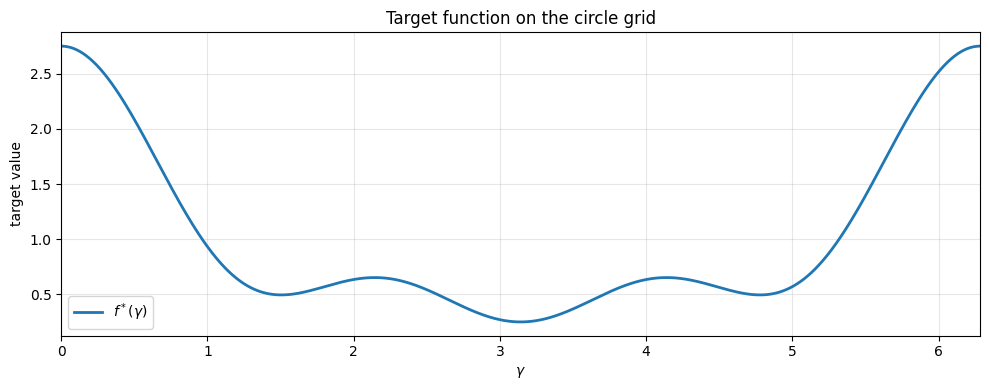
\includegraphics[width=\linewidth]{images/target.png}
		\end{column}
		\begin{column}{0.49\textwidth}
			\centering
			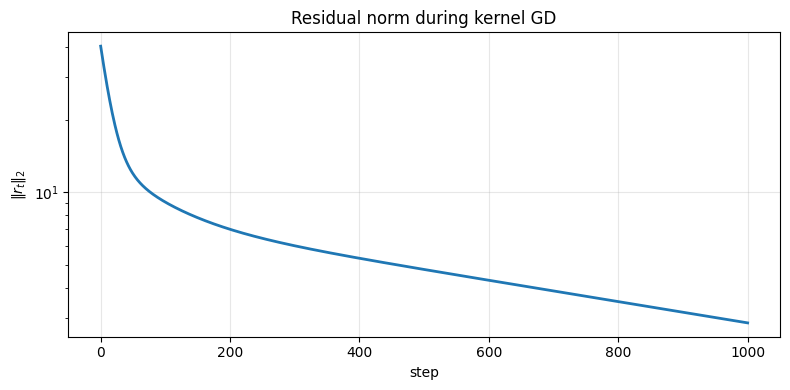
\includegraphics[width=\linewidth]{images/residual_loss.png}
		\end{column}
	\end{columns}

	\vspace{0.3em}
	\small
	\begin{itemize}
		\item Left: target function on the circle grid. $
			      f^{*}(\gamma)
			      =
			      1
			      + 0.9 \cos(\gamma)
			      + 0.5 \cos(2\gamma)
			      + 0.35 \cos(3\gamma).
		      $
		\item Right: residual norm decays smoothly under kernel GD.
	\end{itemize}

	\note{
		The target is a low-dimensional Fourier mixture on the circle.
		The residual norm plot shows stable convergence under the kernel dynamics.
	}
\end{frame}

% ------------------------------------------------------------
\begin{frame}{Empirical spectrum vs continuum prediction}
	\centering
	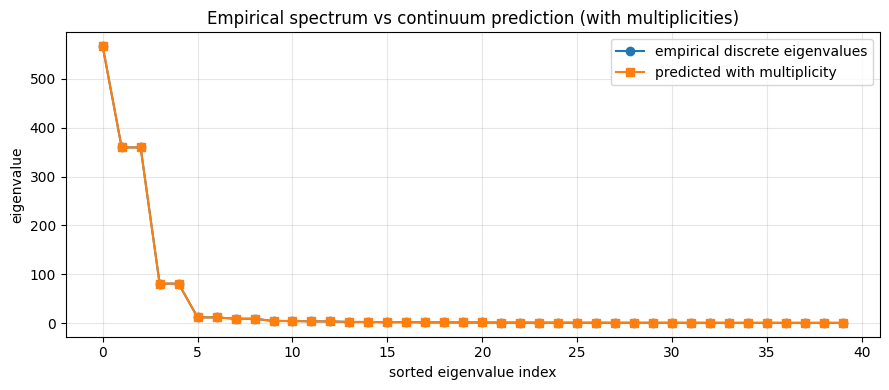
\includegraphics[width=0.9\linewidth]{images/empirical_and_ideal_spectrum.png}

	\vspace{0.3em}
	\small
	The empirical NTK spectrum matches the continuum prediction well once the multiplicity of Fourier modes is accounted for.

	\note{
		On the circle, k >= 1 has multiplicity 2 because of sine/cosine pairs.
		After including that multiplicity, the spectrum matches very well.
	}
\end{frame}

% ------------------------------------------------------------
\begin{frame}{Mode-wise decay}
	\begin{columns}[T,onlytextwidth]
		\begin{column}{0.49\textwidth}
			\centering
			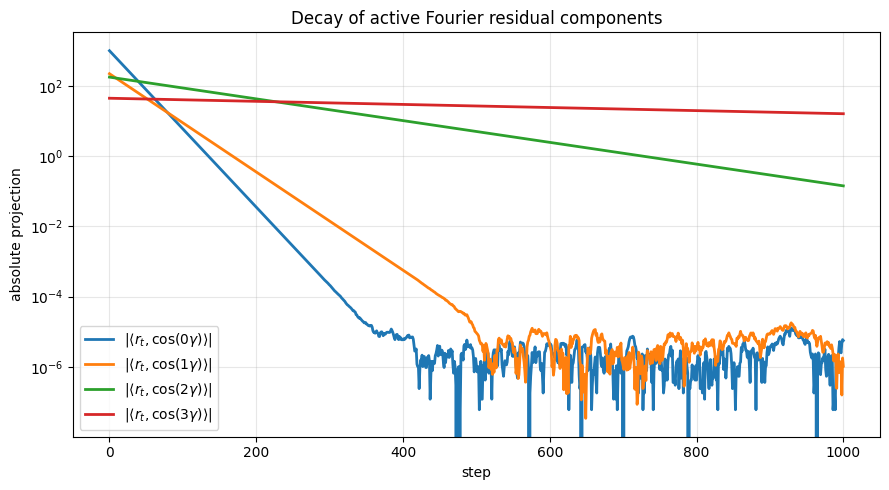
\includegraphics[width=\linewidth]{images/mode_wise_decay.png}
		\end{column}
		\begin{column}{0.49\textwidth}
			\centering
			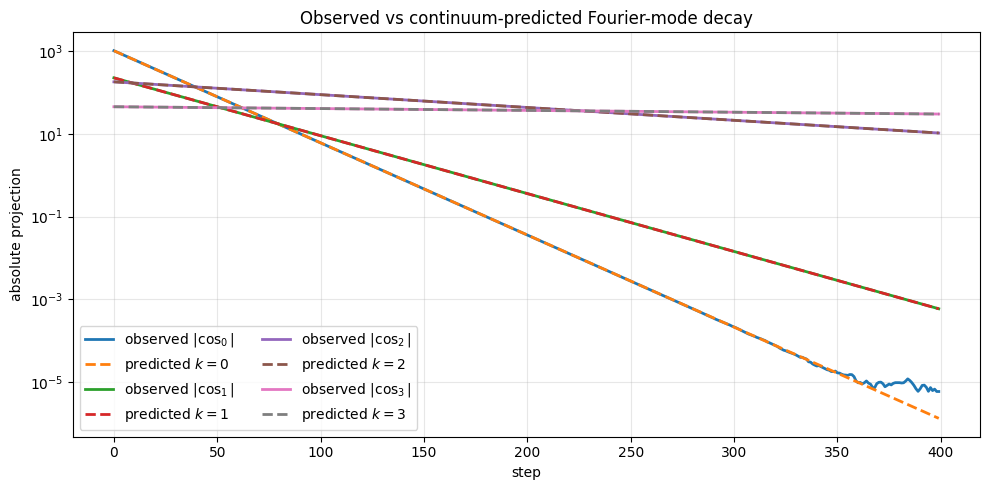
\includegraphics[width=\linewidth]{images/observed_vs_predicted_decay.png}
		\end{column}
	\end{columns}

	\vspace{0.3em}
	\small
	\begin{itemize}
		\item Left: observed decay of the active residual components.
		\item Right: observed decay compared with the ideal rate predicted by the spectrum.
	\end{itemize}

	\note{
		Important subtlety: in discrete time the exact law is geometric,
		alpha_k(t) = (1 - eta lambda_k)^t alpha_k(0).
		For small eta this looks exponential.
		The slower modes look almost flat simply because their eigenvalues are much smaller.
	}
\end{frame}

% ------------------------------------------------------------
\begin{frame}{Current takeaways}
	\small
	\begin{itemize}
		\item The analytic full-NTK kernel on $S^1$ is implemented and numerically consistent.
		\item Kernel regression with NTK dynamics produces the expected residual decay.
		\item The empirical spectrum matches the continuum Fourier prediction on an evenly spaced grid.
		\item Mode-wise decay follows the spectral prediction:
		      lower-frequency / larger-eigenvalue components decay faster.
	\end{itemize}

	\medskip
	\textbf{Next steps}
	\begin{itemize}
		\item Initialization of predictions given by the GP / NNGP limit:
		      \[
			      y_{\mathrm{pred},0} \sim \mathcal{N}(0, K_{0,XX}).
		      \]
		\item Move from theory-validation runs to sampled finite-$n$ experiments.
	\end{itemize}

	\note{
		This is the short message for the meeting:
		the theory-validation pipeline is now working.
		The next natural step is to vary initialization and kernel choice,
		and then move to more realistic sampled-data runs.
	}
\end{frame}

\end{document}
